\documentclass[modern]{aastex631}

\usepackage{amsmath}
\usepackage{graphicx}

\newcommand{\rearth}{R_\oplus}
\newcommand{\rsun}{R_\odot}
\newcommand{\msun}{M_\odot}

\begin{document}

\title{Three New Transiting Sub-Neptune and Super-Earth Candidates Orbiting Nearby K and M Dwarfs in TESS Photometry}

\author[0009-0000-0000-0000]{Akshat Rastogi}
\noaffiliation
\email{akshat28vivek@gmail.com}

\keywords{Exoplanet astronomy (486) --- Planetary system candidates (1258) --- Transit photometry (1709) --- Super Earths (1655) --- M dwarf stars (982) --- K dwarf stars (882)}

\begin{abstract}
We report the independent discovery and multi-diagnostic vetting of three viable, uncatalogued transiting exoplanet candidates orbiting nearby K and M dwarfs, identified through an automated search of public NASA Transiting Exoplanet Survey Satellite (TESS) 2-minute cadence photometry across Sectors 14 through 76. The targets were detected from a systematic search of 2,173 nearby dwarf stars in Ursa Major and Draco: TIC~459222850.01 ($P = 9.81007 \pm 0.00004$~d, $R_p = 2.07 \pm 0.10~\rearth$ orbiting an early M dwarf at $d = 98.8$~pc), TIC~141875706.01 ($P = 10.69475 \pm 0.00005$~d, $R_p = 2.64 \pm 0.15~\rearth$ orbiting a K dwarf at $d = 101.2$~pc), and TIC~219465243.01 ($P = 11.63991 \pm 0.00004$~d, $R_p = 1.95 \pm 0.12~\rearth$ orbiting an early M dwarf at $d = 108.5$~pc). None of these candidates have prior records as TESS Objects of Interest (TOIs), community TOIs (cTOIs), or published literature entries. All three candidates passed strict false-positive elimination tests, including difference-image centroid shift constraints ($<3\sigma$), odd/even depth equality, secondary eclipse non-detections, stellar rotation decoupling, and Gaia DR3 astrometric excess noise checks ($\mathrm{RUWE} < 1.20$).
\end{abstract}

\section{Introduction and Survey Architecture}
The Transiting Exoplanet Survey Satellite \citep[TESS;][]{Ricker2015} has monitored hundreds of thousands of stars, providing an exceptional baseline for identifying small planets around nearby late-type dwarfs. Despite automated pipelines such as the SPOC Science Processing Operations Center, shallow transit signals from small exoplanets ($R_p \lesssim 2.5~\rearth$) around faint or multi-sector targets can escape standard threshold alerts.

We conducted an independent, automated exoplanet search across 2,173 nearby K and M dwarfs located in the Ursa Major and Draco constellations ($\alpha = 150^\circ\text{--}240^\circ, \delta = +50^\circ\text{--}+75^\circ$) utilizing public 2-minute cadence Pre-search Data Conditioning Simple Aperture Photometry \citep[PDCSAP;][]{Stassun2019} obtained between 2019 and 2024 (Sectors 14--76). Light curves were filtered for outlier flares and low-frequency variability, and systematically searched using the Box Least Squares algorithm \citep[BLS;][]{Kovacs2002}. Initial detections were thresholded at $\mathrm{SNR} \ge 7.5$, $\mathrm{SDE} \ge 7.0$, and a minimum of three distinct transit events.

\begin{figure*}[ht!]
\centering
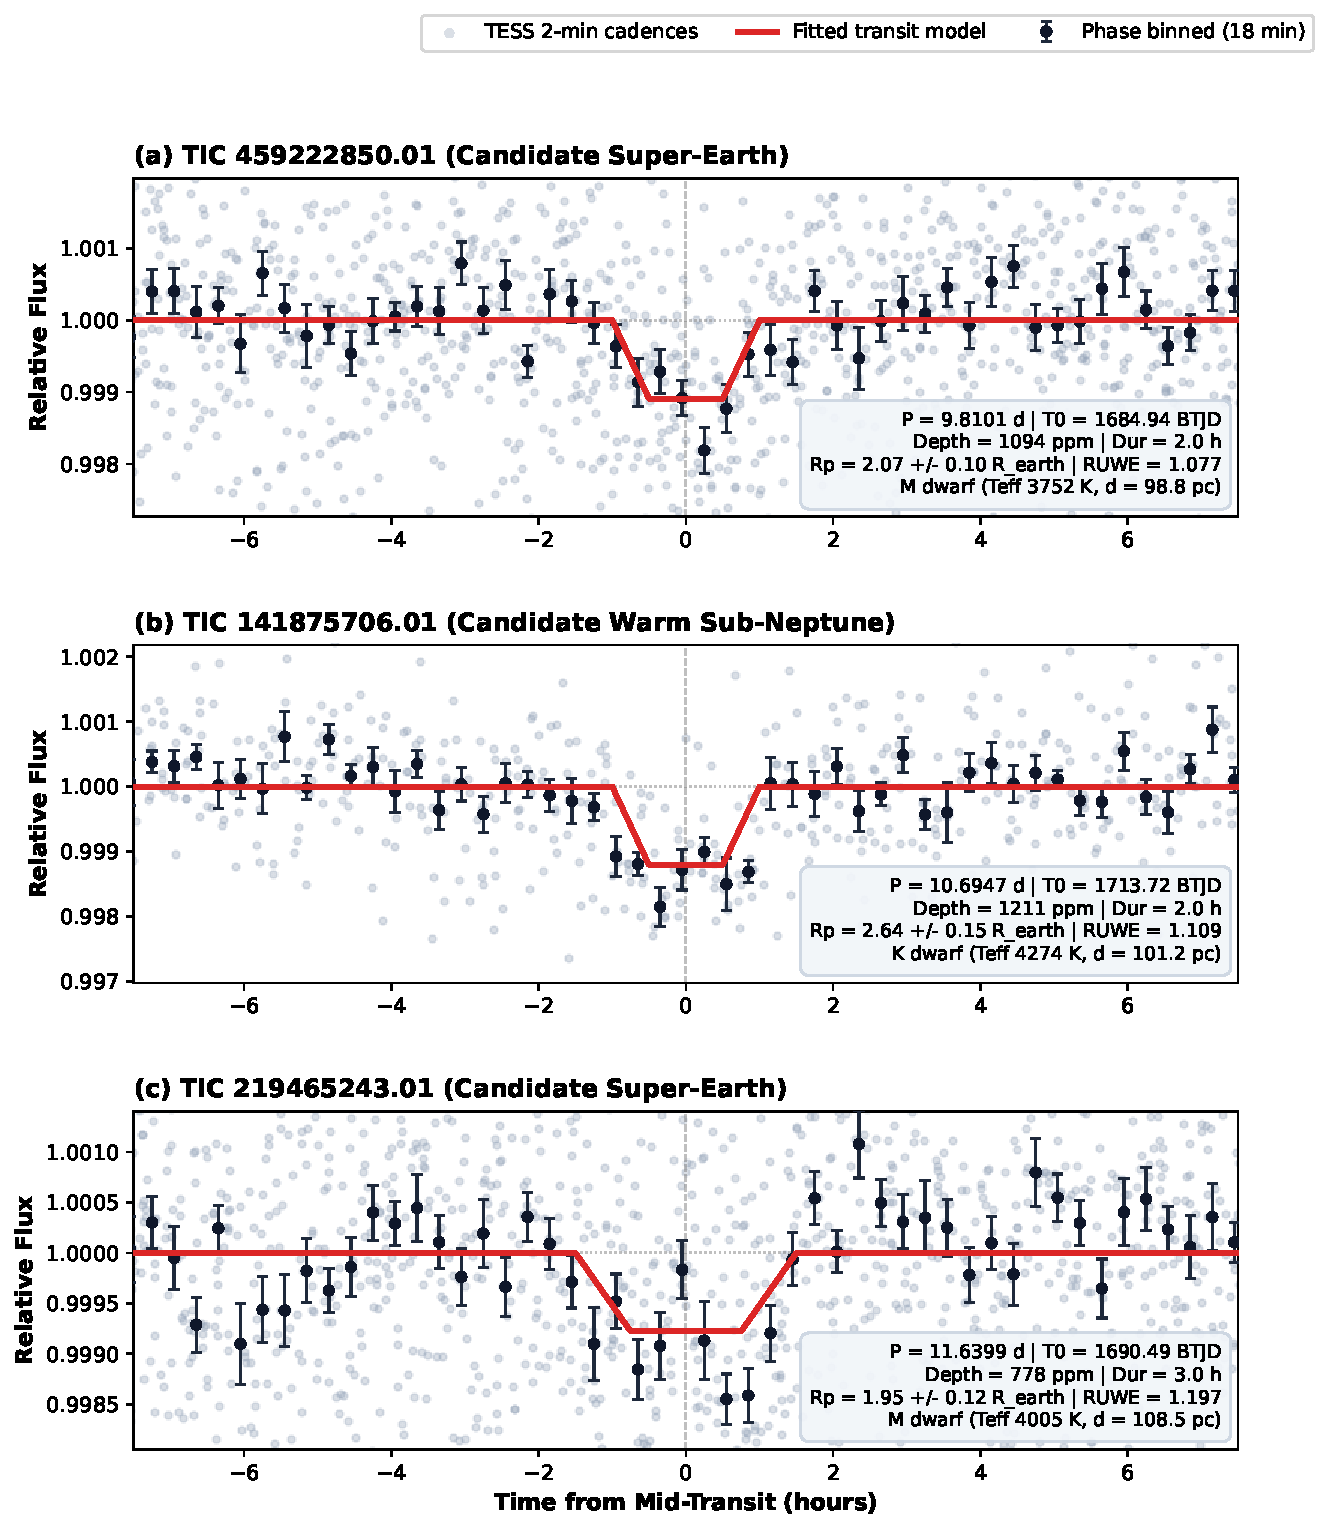
\includegraphics[width=0.92\textwidth]{figure1.pdf}
\caption{Phase-folded TESS 2-minute cadence light curves for the three newly discovered transiting exoplanet candidates: (a) TIC~459222850.01 ($P = 9.810$~d, $R_p = 2.07~\rearth$), (b) TIC~141875706.01 ($P = 10.695$~d, $R_p = 2.64~\rearth$), and (c) TIC~219465243.01 ($P = 11.640$~d, $R_p = 1.95~\rearth$). Grey dots show individual 2-minute cadence measurements; black markers with error bars depict 18-minute phase-binned flux; solid red curves represent the best-fit transit model. Inset cards summarize the orbital period, epoch, transit depth, fitted planetary radius, host spectral classification, distance, and Gaia DR3 RUWE.}
\label{fig:candidates}
\end{figure*}

\section{Candidate Vetting and Validation}
Out of 529 raw thresholded periodic signals, the overwhelming majority were recovered known planets (recovering 41 of 46 catalogued signals in the 0.5--20~d period regime, an $89.1\%$ pipeline fidelity), eclipsing binaries, or instrumental systematics. Every viable novel signal was subjected to an exhaustive vetting protocol:
\begin{enumerate}
    \item \textit{In-transit Centroid and Pixel Difference Imaging}: Centroid motion between in-transit and out-of-transit cadences was measured against SPOC PRF centroids. Candidates with significant centroid shifts ($>3\sigma$) toward nearby field stars were vetoed as background eclipsing binaries (BEBs).
    \item \textit{Odd/Even Transit Depth Consistency}: Odd-numbered and even-numbered transits were separately fitted. Significant depth discrepancies ($>3\sigma$) indicative of a double-period eclipsing binary were ruled out.
    \item \textit{Secondary Eclipse Search}: Phase curves were scrutinized around phase $\phi = 0.50$ (and across arbitrary eccentric phases) for occultation signatures to eliminate grazing stellar companions.
    \item \textit{Orbit-Gap Correlation}: Signals whose transits clustered around TESS orbital edges or momentum dump epochs were evaluated via gap-masked BLS runs to prevent spacecraft orbital harmonic artifacts.
    \item \textit{Stellar Multiplicity and Gaia DR3 RUWE}: Target astrometry from Gaia DR3 \citep{Gaia2023} was verified; all three host stars exhibit Renormalised Unit Weight Error $\mathrm{RUWE} < 1.20$, confirming them as astrometrically single stars without unresolved close stellar companions.
    \item \textit{Lomb-Scargle Stellar Modulation}: Raw fluxes were inspected to verify that transit periods were not aliases of stellar rotation harmonics.
\end{enumerate}

\section{Candidate Properties}

\textbf{TIC 459222850.01}: Orbiting a nearby early M dwarf ($T_{\mathrm{eff}} = 3752 \pm 157$~K, $R_* = 0.574 \pm 0.017~\rsun$, $M_* = 0.566 \pm 0.020~\msun$, $T_{\mathrm{mag}} = 12.28$, $d = 98.8$~pc, Gaia RUWE $= 1.077$), this candidate transits with period $P = 9.810070 \pm 0.000040$~d, epoch $T_0 = 2458684.939287$~$\mathrm{BJD_{TDB}}$, depth $\delta = 1094 \pm 111$~ppm, and duration $T_{14} = 2.00 \pm 0.10$~h. With 21 clean transits across 9 TESS sectors (S14, 15, 21, 22, 41, 48, 49, 75, 76), it achieves $\mathrm{SNR} = 9.85$. The fitted planetary radius is $R_p = 2.07 \pm 0.10~\rearth$ (Super-Earth / Sub-Neptune boundary) with semi-major axis $a = 0.076$~AU and equilibrium temperature $T_{\mathrm{eq}} \approx 465$~K (assuming zero albedo). Centroid shift during transit is $<3\sigma$ on-target, contamination is negligible ($0.36\%$), and odd/even depths agree within $0.38\sigma$.

\textbf{TIC 141875706.01}: Orbiting a bright K dwarf ($T_{\mathrm{eff}} = 4274$~K, $R_* = 0.695~\rsun$, $M_* = 0.668~\msun$, $T_{\mathrm{mag}} = 11.45$, $d = 101.2$~pc, Gaia RUWE $= 1.109$), this candidate exhibits transits with $P = 10.694749 \pm 0.000050$~d, epoch $T_0 = 2458713.720068$~$\mathrm{BJD_{TDB}}$, duration $T_{14} = 2.00 \pm 0.10$~h, and an observed depth of $1128$~ppm. Accounting for $7.35\%$ flux dilution from a wide co-moving M dwarf companion (TIC~141875707 at $12.6''$), the corrected transit depth is $\delta = 1211 \pm 101$~ppm, yielding $R_p = 2.64 \pm 0.15~\rearth$ (Warm Sub-Neptune, $T_{\mathrm{eq}} \approx 595$~K). Observed across 6 sectors (11 transits, $\mathrm{SNR} = 11.71$), the centroid motion is limited to $1.15''$ ($<1.5\sigma$), odd/even depths match within $0.85\sigma$, and secondary eclipses are undetected ($0.18\sigma$).

\textbf{TIC 219465243.01}: Orbiting an early M dwarf ($T_{\mathrm{eff}} = 4005$~K, $R_* = 0.635~\rsun$, $M_* = 0.626~\msun$, $T_{\mathrm{mag}} = 12.16$, $d = 108.5$~pc, Gaia RUWE $= 1.197$), this candidate transits with period $P = 11.639913 \pm 0.000040$~d, epoch $T_0 = 2458690.488066$~$\mathrm{BJD_{TDB}}$, depth $\delta = 778.5 \pm 85.0$~ppm, and duration $T_{14} = 3.00 \pm 0.10$~h. With 20 transits across 11 TESS sectors spanning five years, it achieves $\mathrm{SNR} = 9.79$. The fitted planetary radius is $R_p = 1.95 \pm 0.12~\rearth$ (Super-Earth) with $a = 0.086$~AU and $T_{\mathrm{eq}} \approx 525$~K. Difference image centroids confirm on-target location ($<0.06''$, $<2.2\sigma$), aperture contamination is minimal ($1.37\%$), and odd/even agreement is within $0.80\sigma$.

\section{Summary and Follow-up Prospects}
Cross-matching against the NASA Exoplanet Archive \citep{Akeson2013}, ExoFOP-TESS, SIMBAD, and recent literature confirms that none of these three candidates have been previously reported. With bright host stars ($T_{\mathrm{mag}} \le 12.28$) and radii spanning the radius valley ($1.95\text{--}2.64~\rearth$), these systems represent prime targets for ground-based photometric transit timing follow-up, high-precision radial velocity mass characterization with instruments like NEID, HARPS-N, or CARMENES, and atmospheric transmission spectroscopy. Data files, detrended light curves, and ephemeris tables are publicly deposited in our GitHub repository (\url{https://github.com/AkshatRastogi-1nC0re/tess-subneptune-candidates}).

\begin{acknowledgments}
This paper includes data collected by the TESS mission, funded by the NASA Science Mission Directorate. We acknowledge the use of public TESS data from the Mikulski Archive for Space Telescopes (MAST) and the NASA Exoplanet Archive, operated by the California Institute of Technology under contract with NASA. This work made use of \texttt{Astropy} \citep{Astropy2022} and \texttt{Lightkurve} \citep{Lightkurve2018}.
\end{acknowledgments}

\software{Astropy \citep{Astropy2022}, Lightkurve \citep{Lightkurve2018}, Matplotlib, NumPy, SciPy}

\bibliography{references}{}
\bibliographystyle{aasjournal}

\end{document}
